\subsection{Gestión de usuarios y Directorio Activo}

En la administración de sistemas informáticos, la gestión de usuarios es un componente esencial para asegurar el correcto funcionamiento y la seguridad de la infraestructura tecnológica de una organización. El AD es una herramienta crucial en este ámbito, ya que permite la centralización y automatización de la gestión de usuarios, dispositivos y recursos \autocite{thakur_user_2015-1,josang_local_2015}. Este epígrafe aborda los conceptos fundamentales de la gestión de usuarios, las ventajas y características del AD, así como su implementación y administración.

Un AD es una base de datos central que se utiliza para administrar y organizar los recursos de una red de computadoras. La gestión de usuarios es una función importante en un AD, ya que permite crear, eliminar y editar los perfiles de los usuarios en un dominio. Además, también implica la asignación de permisos y roles, que determinan el nivel de acceso y las acciones que cada usuario puede realizar en la red \autocite{bartlett_samba_2005,dansimp_active_2023,imanudin_active_2019,allen_active_2003}.

En la \autoref{fig:ad-tree-example} extraída de \autocite{carter_ldap_2003} a continuación se muestra como se organizan jerárquicamente los recursos dentro de un AD.

\begin{figure}[H]
    \centering
    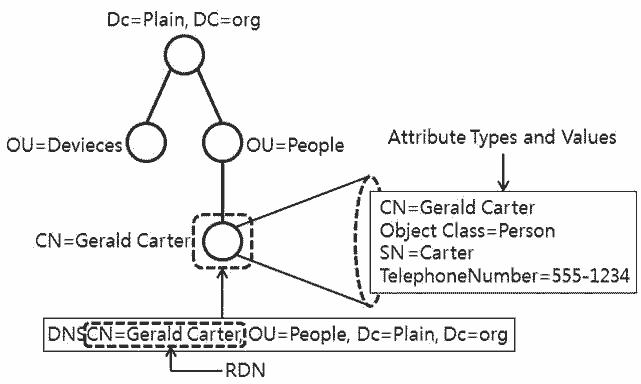
\includegraphics[width=\linewidth]{images/ad-tree-2.png}
    \caption{Organización jerárquica de recursos en un AD}
    \label{fig:ad-tree-example}
\end{figure}

El esquema de AD contiene definiciones formales de cada clase de objeto que se puede crear en un directorio. Por ejemplo, en el caso de los usuarios, el esquema define atributos como el nombre, apellido, nombre para mostrar, nombre de inicio de sesión, dirección de correo electrónico, número de teléfono \autocite{harrison_lightweight_2006,voglmaier_abcs_2003,howes_ldap_1997,shlipsey3_how_2024}. En la \autoref{table:ad-user-schema-attributes} se muestran algunos atributos del esquema de usuario de un AD, así como ejemplos de valores que pueden tomar estos atributos \autocite{derdus_user_2024}.

\begin{longtable}{|l|p{5cm}|p{5cm}|}
    \caption{Algunos atributos del esquema de usuario en el AD}
    \label{table:ad-user-schema-attributes}                                                                                                        \\
    \hline
    \textbf{Atributo} & \textbf{Descripción}                                                      & \textbf{Ejemplo}                               \\
    \hline
    \endfirsthead
    \hline
    displayName       & Nombre para mostrar del usuario, puede ser diferente al nombre real       & Juan Pérez                                     \\
    \hline
    distinguishedName & Nombre único del objeto en el directorio, incluye la ruta completa        & CN=jperez, OU=Dirección, DC=ejemplo, DC=com    \\
    \hline
    givenName         & Nombre del usuario                                                        & Juan                                           \\
    \hline
    mail              & Dirección de correo electrónico del usuario                               & juan.perez@ejemplo.com                         \\
    \hline
    objectSid         & Identificador de seguridad (SID) del usuario                              & S-1-5-21-1234567890-1234567890-1234567890-1234 \\
    \hline
    sAMAccountName    & Nombre de inicio de sesión compatible con versiones anteriores de Windows & jperez                                         \\
    \hline
    sn                & Apellido del usuario                                                      & Pérez                                          \\
    \hline
    telephoneNumber   & Número de teléfono del usuario                                            & +34 123 456 789                                \\
    \hline
    userPrincipalName & Nombre de inicio de sesión del usuario                                    & jperez@ejemplo.com                             \\
    \hline
\end{longtable}
